\documentclass[12pt]{report}
\usepackage[utf8]{inputenc}
\usepackage[russian]{babel}
%\usepackage[14pt]{extsizes}
\usepackage{listings}

% Для листинга кода:
\lstset{ %
language=python,                 % выбор языка для подсветки (здесь это С)
basicstyle=\small\sffamily, % размер и начертание шрифта для подсветки кода
numbers=left,               % где поставить нумерацию строк (слева\справа)
numberstyle=\tiny,           % размер шрифта для номеров строк
stepnumber=1,                   % размер шага между двумя номерами строк
numbersep=5pt,                % как далеко отстоят номера строк от подсвечиваемого кода
showspaces=false,            % показывать или нет пробелы специальными отступами
showstringspaces=false,      % показывать или нет пробелы в строках
showtabs=false,             % показывать или нет табуляцию в строках
frame=single,              % рисовать рамку вокруг кода
tabsize=2,                 % размер табуляции по умолчанию равен 2 пробелам
captionpos=t,              % позиция заголовка вверху [t] или внизу [b] 
breaklines=true,           % автоматически переносить строки (да\нет)
breakatwhitespace=false, % переносить строки только если есть пробел
escapeinside={\#*}{*)}   % если нужно добавить комментарии в коде
}

% Для измененных титулов глав:
\usepackage{titlesec, blindtext, color} % подключаем нужные пакеты
\definecolor{gray75}{gray}{0.75} % определяем цвет
\newcommand{\hsp}{\hspace{20pt}} % длина линии в 20pt
% titleformat определяет стиль
\titleformat{\chapter}[hang]{\Huge\bfseries}{\thechapter\hsp\textcolor{gray75}{|}\hsp}{0pt}{\Huge\bfseries}


% plot
\usepackage{pgfplots}
\usepackage{filecontents}
\usetikzlibrary{datavisualization}
\usetikzlibrary{datavisualization.formats.functions}

\begin{document}
 
%\def\chaptername{} % убирает "Глава"
\begin{titlepage}
	\centering
	{\scshape\LARGE МГТУ им. Баумана \par}
	\vspace{3cm}
	{\scshape\Large Лабораторная работа №5\par}
	\vspace{0.5cm}	
	{\scshape\Large По курсу: "Операционные системы"\par}
	\vspace{1.5cm}
	{\huge\bfseries Взаимодействие параллельных процессов\par}
	\vspace{2cm}
	\Large Работу выполнил: студент группы ИУ7-53Б Наместник Анастасия\par
	\vspace{0.5cm}
	\Large Преподаватель:  Рязанова Н. Ю.\par

	\vfill
	\large \textit {Москва, 2020} \par
\end{titlepage}

\newpage

На листингах 1,...,4 представлена первая программа, демонстрирующая реализацию задачи «Производство-потребление» по алгоритму Э. Дейкстры.

\begin{lstlisting}[label=some-code,caption=Начальные установки]
#define N 24 //buffer size
#define LETTERS "abcdefghijklmnopqrstuvwxyz"
#define OBJECT_QTY 1
#define PROC_COUNT 3

#define BS 0 //bin_sem
#define BF 1 //buffer_full
#define BE 2 //buffer_empty

#define P -1
#define V 1

struct sembuf producerStart[2] = {{BE, P, 0}, {BS, P, 0}};
struct sembuf producerStop [2] = {{BS, V, 0}, {BF, V, 0}};
struct sembuf consumerStart[2] = {{BF, P, 0}, {BS, P, 0}};
struct sembuf consumerStop [2] = {{BS, V, 0}, {BE, V, 0}};

int *prod_pos = NULL;
int *cons_pos = NULL;
char *buff_pos = NULL;

const int size = sizeof(int) * 2 + sizeof(char) * N;
\end{lstlisting}

\begin{lstlisting}[label=some-code,caption=Код подпрограммы main()]
int main()
{
    srand(time(NULL));
    
    printf("Parent: PID = %d\n", getpid());
    
    int shm_perms = S_IRUSR | S_IWUSR | S_IRGRP | S_IROTH;
    int fd = shmget(IPC_PRIVATE, size, shm_perms);
    if (fd == -1)
    {
        perror("New shared memory segment could not be created\n");
        return 1;
    }
    
    int *addr = shmat(fd, NULL, 0);
    if ((char *)addr == (char*) -1)
    {
        perror("Shared memory segment could not be attached to the address space of the calling process\n");
        return 1;
    }
    
    prod_pos = addr;
    cons_pos = addr + sizeof(int);
    buff_pos = (char *)(addr + sizeof(int) * 2);
    
    *prod_pos = 0;
    *cons_pos = 0;

    int sem_perms = S_IRUSR | S_IWUSR | S_IRGRP | S_IROTH;
    int semid = semget(IPC_PRIVATE, 3, IPC_CREAT | IPC_EXCL | sem_perms);
    if (semid == -1)
    {
        perror("New semaphore set could not be created\n");
        return 1;
    }
    
    int init_BS = semctl(semid, BS, SETVAL, 1);
    if (init_BS == -1)
    {
        perror("SETVAL command could not be applied to semaphore BS\n");
        return 1;
    }

    int init_BF = semctl(semid, BF, SETVAL, 0);
    if (init_BF == -1)
    {
        perror("SETVAL command could not be applied to semaphore BF\n");
        return 1;
    }

    int init_BE = semctl(semid, BE, SETVAL, N);
    if (init_BE == -1)
    {
        perror("SETVAL command could not be applied to semaphore BE\n");
        return 1;
    }

    for (int i = 0; i < PROC_COUNT; i++)
    {
        ProducerCreation(semid, i);
        ConsumerCreation(semid, i);
    }
    
    int status;
    for (int i = 0; i < PROC_COUNT * 2; i++)
        wait(&status);
    
    if (shmdt(addr) == -1)
        perror("Shared memory segment could not be detached from the address space of the calling process\n");
    return 0;
}
\end{lstlisting}

\begin{lstlisting}[label=some-code,caption=Код подпрограмм создания и работы производителя]
void ProducerRoutine(const int semid, const int prod_id)
{
    //Random delays
    sleep(rand() % 2);
    
    if (semop(semid, producerStart, 2) == -1)
    {
        perror("Producer's semop failed (couldn't enter the critical zone)\n");
        exit(1);
    }
    printf("Producer with id = %d is in the critical zone\n", prod_id);
    
    buff_pos[*prod_pos] = LETTERS[*prod_pos];
    
    printf("Producer with id = %d posed at %d produced %c\n", prod_id, *prod_pos, buff_pos[*prod_pos]);
    (*prod_pos)++;
    
    if (semop(semid, producerStop, 2) == -1)
    {
        perror("Producer's semop failed (couldn't escape the critical zone)\n");
        exit(1);
    }
}

void ProducerCreation(const int semid, const int id)
{
    int process;
    if ((process = fork()) == -1)
    {
        perror("Can\'t fork.\n");
        exit(1);
    }
    
    else if (process == 0)
    {
        printf("Producer(child process) with id = %d (PID = %d) was created\n", id, getpid());
        
        ProducerRoutine(semid, id);
    
        printf("Producer with id = %d executed\n\n", id);
        exit(0);
    }
}
\end{lstlisting}

\begin{lstlisting}[label=some-code,caption=Код подпрограмм создания и работы потребителя]
void ConsumerRoutine(const int semid, const int cons_id)
{
    //Random delays
    sleep(rand() % 5);
    
    if (semop(semid, consumerStart, 2) == -1)
    {
        perror("Consumer's semop failed (couldn't enter the critical zone)\n");
        exit(1);
    }
    
    printf("Consumer with id = %d posed at %d consumed %c\n", cons_id, *cons_pos, buff_pos[*cons_pos]);
    (*cons_pos)++;

    if (semop(semid, consumerStop, 2) == -1)
    {
        perror("Consumer's semop failed (couldn't escape the critical zone)\n");
        exit(1);
    }
}

void ConsumerCreation(const int semid, const int id)
{
    int process;
    if ((process = fork()) == -1)
    {
        perror("Can\'t fork.\n");
        exit(1);
    }
    
    else if (process == 0)
    {
        printf("Consumer(child process) with id = %d (PID = %d) was created\n", id, getpid());
    
        ConsumerRoutine(semid, id);

        printf("Consumer with id = %d executed\n\n", id);
        exit(0);
    }
}
\end{lstlisting}

На рисунке 1 приведен результат работы программы, в случае когда диапазон задержек выполнения потребителей больше диапазона задержек выполнения производителей. 
При этом задержки потребителей случайным образом принимают следующие значения: 0, 1, 2, 3, 4, - а задержки производителей - 0, 1. 
Следовательно, производство осуществляется быстрее потребления.
\begin{center}
		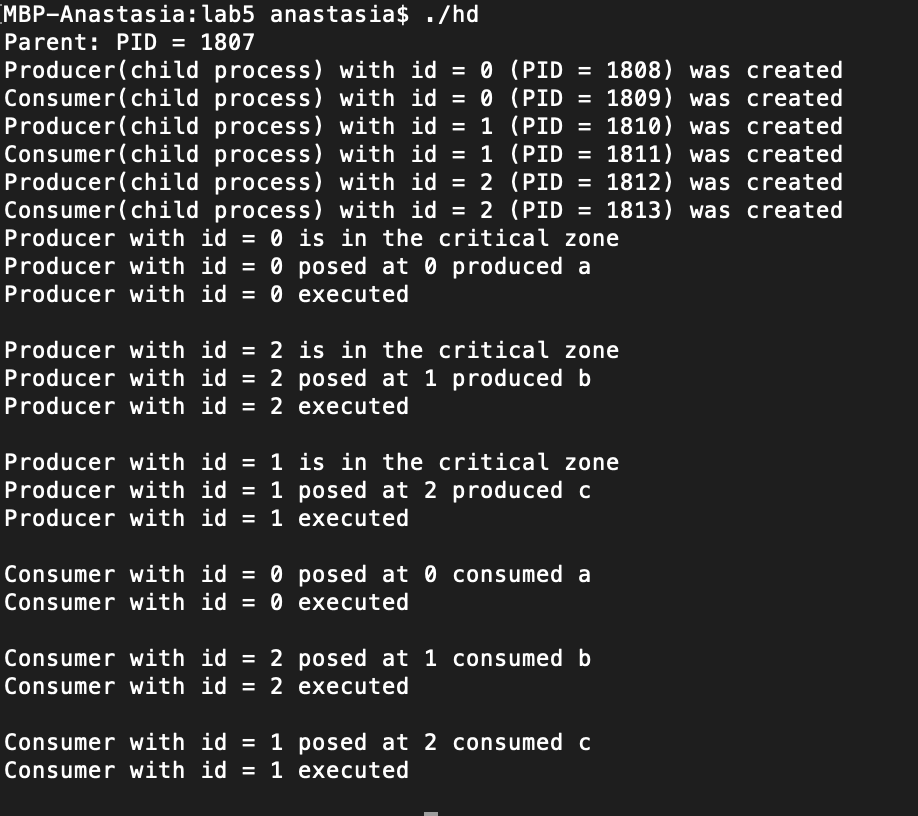
\includegraphics[scale=0.8]{pics/Cns_is_slower.png}
		
			Рис 1:  Результат работы программы (задержки потребителей больше)
\end{center}

На листингах 5,...,8 представлена вторая программа, демонстрирующая реализацию задачи «Читатели – писатели» по монитору Хоара с четырьмя функциями: Начать\_чтение, Закончить\_чтение, Начать\_запись, Закончить\_запись.

\begin{lstlisting}[label=some-code,caption=Начальные установки]
#include <sys/types.h>
#include <sys/ipc.h>
#include <sys/sem.h>
#include <sys/stat.h>
#include <sys/shm.h>
#include <stdlib.h>
#include <unistd.h>

#include <pthread.h>
#include <stdio.h>

#define WHITE "\033[0m"
#define GREEN "\033[0;32m"

#define WRITERS 5
#define READERS 3
#define FLG 0

#define AW 0 //active_writer (logical)
#define AR 1 //active_readers
#define QW 2 //writers_queue
#define QR 3 //readers_queue

#define D -1 //decrement
#define I 1 //increment
#define W 0 //wait (sleep()) while semaphore is not 0

struct sembuf start_read[5] = {
    {QR, I, FLG},   //readers_queue + 1 
    {QW, W, FLG},   //wait until writers_queue = 0
    {AW, W, FLG},   //wait until active_writer = 0
    {QR, D, FLG},   //readers_queue - 1
    {AR, I, FLG}};  //active_readers + 1
struct sembuf stop_read[1] = {{AR, D, FLG}};
struct sembuf start_write[5] = {
    {QW, I, FLG},  //writers_queue + 1 
    {AR, W, FLG},  //wait until active_readers = 0
    {AW, W, FLG},  //wait until active_writer = 0
    {AW, I, FLG},  //active_writer = 1
    {QW, D, FLG}   //writers_queue - 1 
};
struct sembuf stop_write[1] = {{AW, D, FLG}}; //active_writer = 0

int *addr = NULL;
\end{lstlisting}

\begin{lstlisting}[label=some-code,caption=Код подпрограммы main()]
int main()
{
    printf("Parent: PID = %d\n", getpid());

    int shm_perms = S_IRUSR | S_IWUSR | S_IRGRP | S_IROTH;
    int fd = shmget(IPC_PRIVATE, sizeof(int), shm_perms);
    if (fd == -1)
    {
        perror("New shared memory segment could not be created\n");
        return 1;
    }

    addr = shmat(fd, NULL, 0);
    if ((char *)addr == (char*) -1)
    {
        perror("Shared memory segment could not be attached to the address space of the calling process\n");
        return 1;
    }
    
    *addr = 0;

    int sem_perms = S_IRUSR | S_IWUSR | S_IRGRP | S_IROTH;
    int semid = semget(IPC_PRIVATE, 4, IPC_CREAT | IPC_EXCL | sem_perms);
    if (semid == -1)
    {
        perror("New semaphore set could not be created\n");
        return 1;
    }
    
    for (int i = 0; i < WRITERS; i++)
        Writer(semid, i);
    
    for (int i = 0; i < READERS; i++)
        Reader(semid, i);
    
    int status;

    for (int i = 0; i < WRITERS + READERS; i++)
        wait(&status);
   
    if (shmdt(addr) == -1)
        perror("Shared memory segment could not be detached from the address space of the calling process\n");
    return 0;
}
\end{lstlisting}

\begin{lstlisting}[label=some-code,caption=Код подпрограммы Writer() - процесс писатель]
void Writer(const int semid, const int id)
{
    int process;
    if ((process = fork()) == -1)
    {
        perror("Can\'t fork.\n");
        exit(1);
    }
    
    else if (process == 0)
    {
        while(1)
        {
            if (semop(semid, start_write, 5) == -1)
            {
                perror("Writer's semop failed (couldn't enter the critical zone)\n");
                exit(1);
            }
            
            (*addr)++;
            printf("%sWriter(child process) with id = %d (PID = %d) wrote %d\n", GREEN, id, getpid(), *addr);
            
            if (semop(semid, stop_write, 1) == -1)
            {
                perror("Writer's semop failed (couldn't escape the critical zone)\n");
                exit(1);
            }
            sleep(2);
        }
        exit(0);
    }
}
\end{lstlisting}

\begin{lstlisting}[label=some-code,caption=Код подпрограммы Reader() - процесс читатель]
void Reader(const int semid, const int id)
{
    int process;
    if ((process = fork()) == -1)
    {
        perror("Can\'t fork.\n");
        exit(1);
    }
    
    else if (process == 0)
    {
        while(1)
        {
            if (semop(semid, start_read, 5) == -1)
            {
                perror("Reader's semop failed (couldn't enter the critical zone)\n");
                exit(1);
            }
            
            printf("%sReader(child process) with id = %d (PID = %d) read %d\n", WHITE, id, getpid(), *addr);
            
            if (semop(semid, stop_read,1) == -1)
            {
                perror("Reader's semop failed (couldn't escape the critical zone)\n");
                exit(1);
            }
            sleep(1);
        }
        exit(0);
    }
}
\end{lstlisting}

На рисунке 2 приведен результат работы второй программы.
\begin{center}
		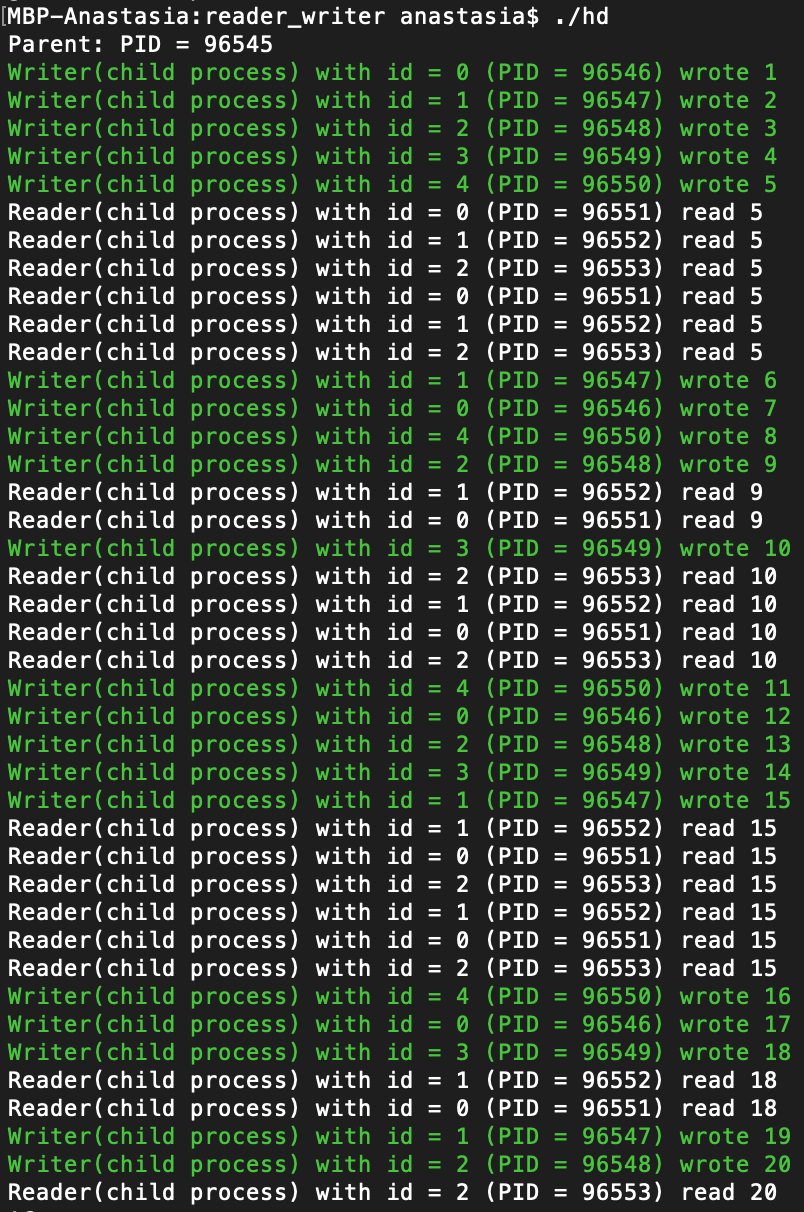
\includegraphics[scale=0.8]{pics/RW.png}
		
			Рис 2.:  Результат работы программы 
\end{center}


\end{document}